\documentclass{beamer}% тип документа
% далее идёт преамбула
\usepackage[T2A]{fontenc}
\usepackage[utf8]{inputenc}
\usepackage[russian]{babel}

%Settings (непонятная хуйня)
\setbeamercolor{itemize item}{fg=black}
\setbeamercolor{itemize subitem}{fg=black}
\setbeamercolor{alerted text}{fg=black}
\setbeamertemplate{itemize items}{\textbullet}% отключает кошмарные синие треугольники
\setbeamerfont*{itemize/enumerate subbody}{parent=itemize/enumerate body}
\setbeamerfont*{itemize/enumerate subsubbody}{parent=itemize/enumerate subbody}
\setbeamerfont{alerted text}{series=\bfseries}
\usepackage{graphics}
\graphicspath{ {./images/} }
\makeatletter
\setlength{\@fptop}{0pt}
\makeatother
\usepackage{pgfplots}
\pgfplotsset{compat=1.9}
\usepackage{hyperref}
%конец непонятной хуйни


\title{Измерение интенсивности радиационного фона}
\author{Аношин Матвей, Масов Егор}

\begin{document}
\begin{frame}
    \titlepage
\end{frame}

\begin{frame}{\textsc{Цели работы и оборудование}}
    \large{\textbf{Цели работы:}}
    \begin{itemize}
        \item \normalsize{применение методов обработки экспериментальных данных для изучения статистических закономерностей при измерении интенсивности радиационного фона}
        \item {обработка экспериментальных данных со счетчика Гейгера-Мюллера с помощью программы STAT}
        \item {обработка экспериментальных данных с помощью фотодиода и осциллографа}
    \end{itemize}
    \vspace{15}
    \large{\textbf{В работе используются:}}\\
    \normalsize{Счетчик Гейгера-Мюллера (СТС-6), блок питания, компьютер с интерфейсом связи со счетчиком, фотодиод, осциллограф _модель_нейм_}
\end{frame}

\begin{frame}{\textsc{Справка о космических лучах}}
    \begin{itemize}
        \item Первичные космические лучи - потоки частиц от взрывов сверхновых (галактическое космическое излучение) и со стороны Солнца.
        \item Вторичные космические лучи - образуются при взаимодействии первичных космических лучей с атмосферой Земли. Состоит из мягкой (фотоны, электроны, позитроны) и жесткой (вторичные протоны и мюоны) компонент.
    \end{itemize}
\end{frame}
    
\begin{frame}{\textsc{Принцип работы счетчика Гейгера}}
    \begin{figure}[t]
            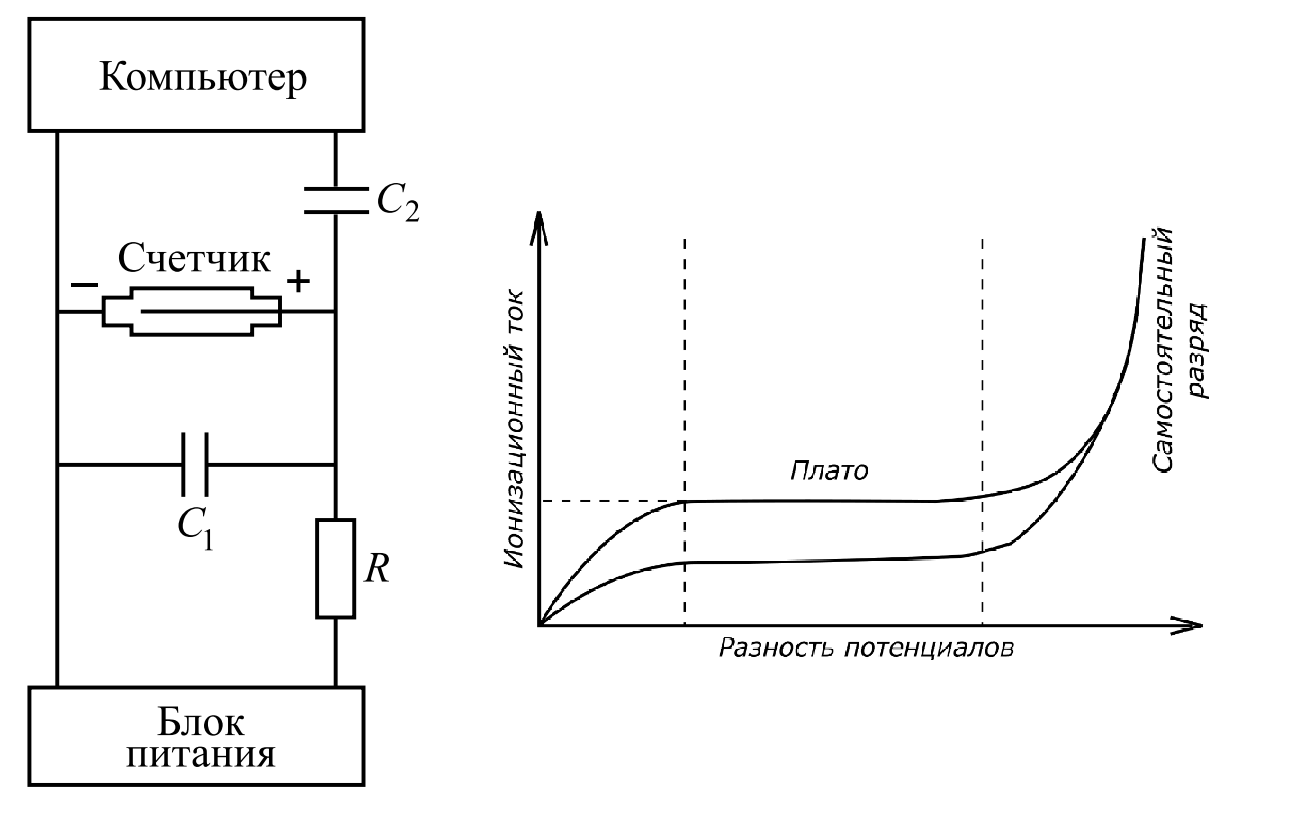
\includegraphics[width=1.1\linewidth, height=220.0]{images/Geiger counter.png}
    \end{figure}
\end{frame}

\begin{frame}{\textsc{Результаты измерений с помощью STAT}}
    \begin{figure}[ht]
        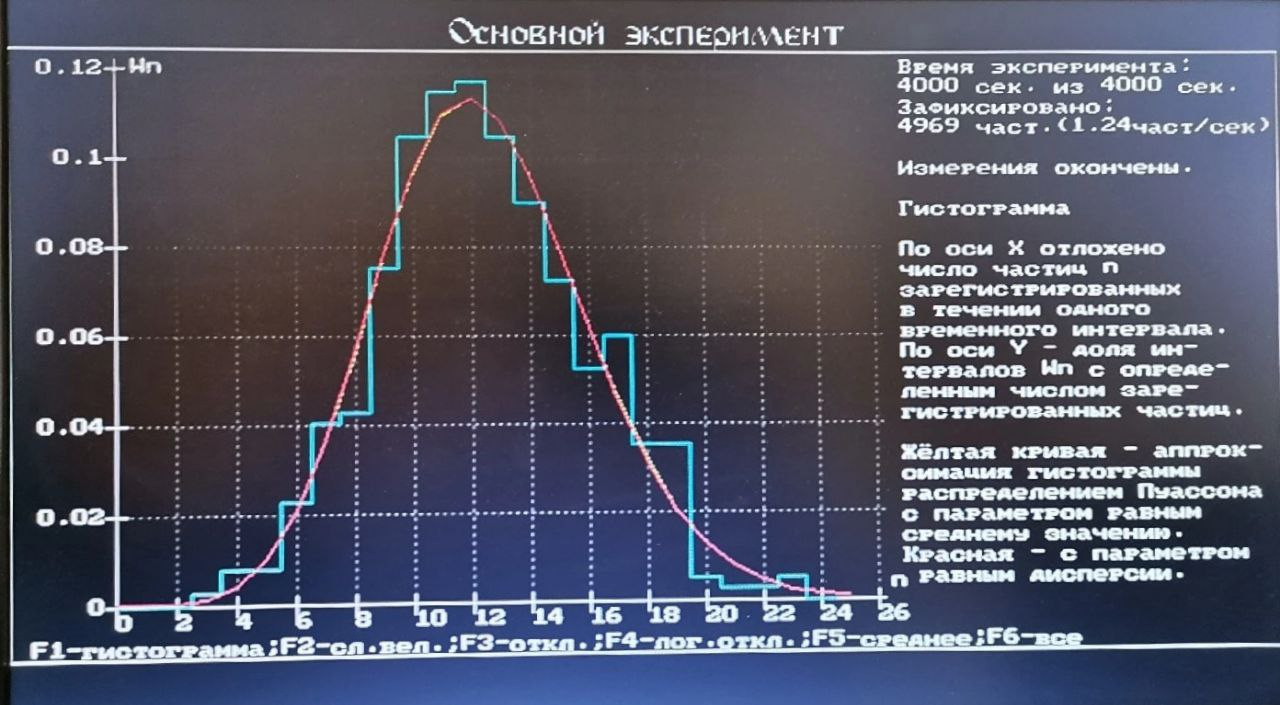
\includegraphics[width=1.0\linewidth]{images/res.jpg}
    \end{figure}
\end{frame}

\begin{frame}{\textsc{Результаты измерений с помощью STAT}}
    \begin{figure}[ht]
        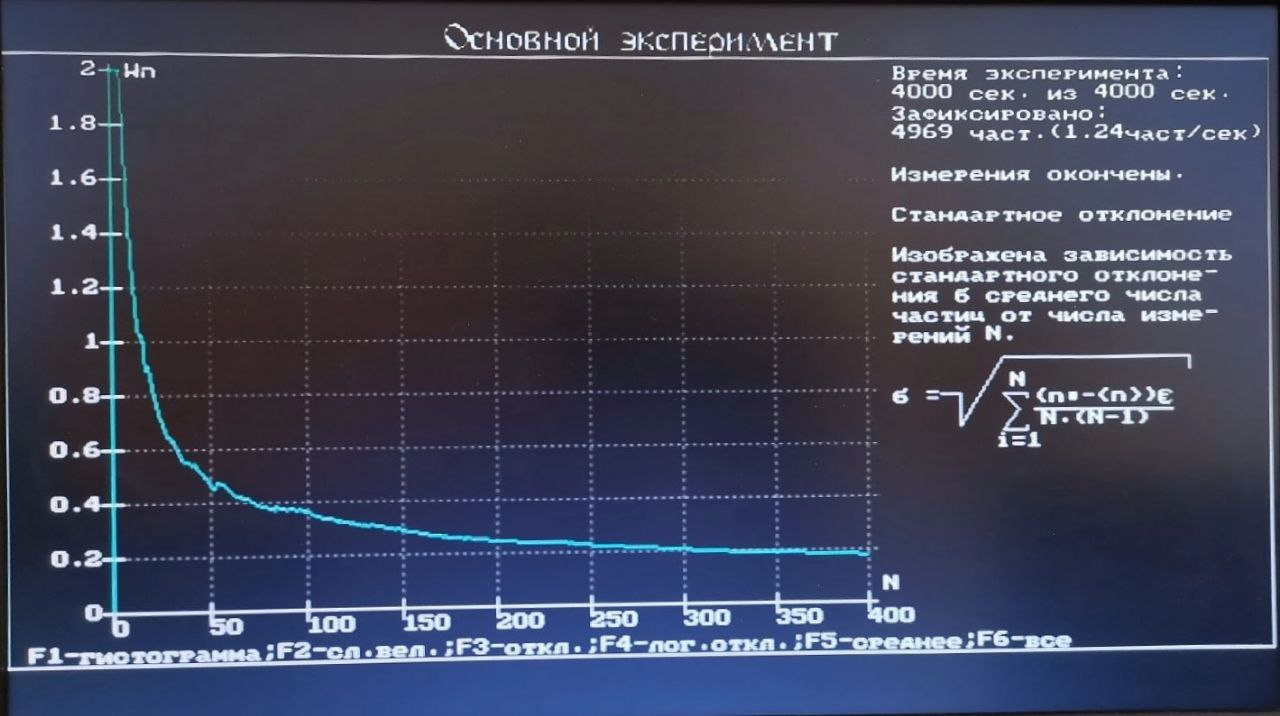
\includegraphics[width=1.0\linewidth]{images/sigma_n.jpg}
    \end{figure}
\end{frame}

\begin{frame}{\textsc{Результаты измерений с помощью STAT}}
    \begin{figure}[h]
        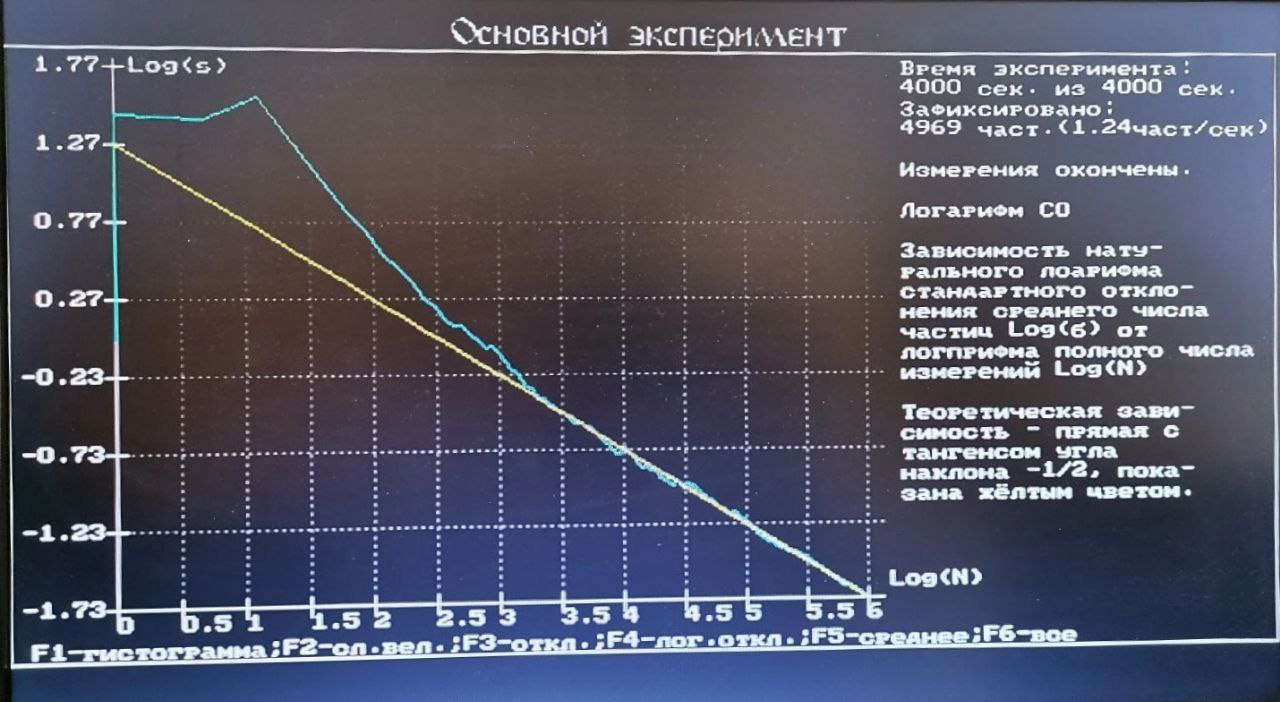
\includegraphics[width=1.0\linewidth]{images/sigma_n_1.jpg}
    \end{figure}
\end{frame}    

\begin{frame}{\textsc{Результаты измерений с помощью STAT}, \tau = 20 }
    \begin{figure}[ht]
        \begin{minipage}{.5\textwidth}
            \begin{table}[t]
                \tabcolsep=0.15cm
                \begin{tabular}{|c | c | c |} 
                    \hline
                    n_2_0   &	w(n_2_0)	&   P_n \\ 
                    \hline
                    11  &	0,005   &	0,001 \\
                    14  &	0,01    &	0,006 \\
                    15  &	0,015   &	0,010 \\
                    16	&   0,02    &	0,016 \\
                    17	&   0,01    &	0,023 \\
                    18	&   0,03    &	0,032 \\
                    19	&   0,03    &	0,042 \\
                    20	&   0,06    &	0,052 \\
                    21	&   0,06    &	0,062 \\
                    22	&   0,11    &	0,070 \\
                    23	&   0,07    &	0,076 \\ [1ex]
                    \hline
                \end{tabular}
            \end{table}
        \end{minipage}%
        \begin{minipage}{.5\textwidth}
            \begin{table}[t]
                \tabcolsep=0.15cm
                \begin{tabular}{|c | c | c |} 
                    \hline
                    n_2_0   &	w(n_2_0)	&   P_n \\ 
                    \hline
                    24	&   0,09    &	0,080 \\
                    25	&   0,05    &	0,080 \\
                    26	&   0,08    &	0,077 \\
                    27	&   0,06    &	0,071 \\
                    28  &	0,09    &	0,063 \\
                    29  &	0,05    &	0,055 \\
                    30  & 	0,07    &	0,045 \\
                    31  &   0,05    &	0,037 \\
                    32  &   0,03    &	0,029 \\
                    33  &	0,03    &	0,022 \\
                    35  &	0,01    & 	0,011 \\
                    36  &	0,01    &	0,008 \\ [1ex]
                    \hline
                \end{tabular}
            \end{table}
        \end{minipage}
    \end{figure}
\end{frame}

\begin{frame}{\textsc{Диаграмма распределения}, \tau = 20}
    \begin{figure}[ht]
        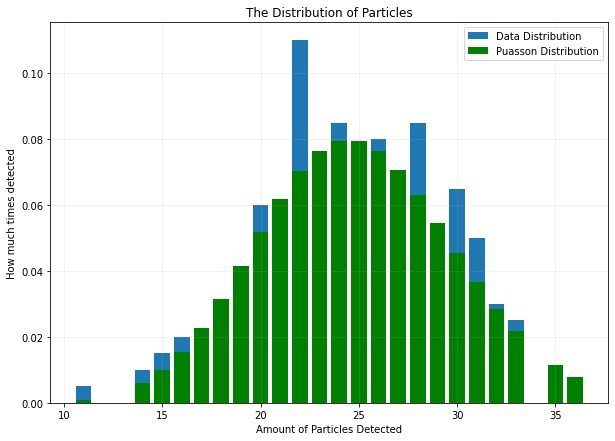
\includegraphics[width=1.0\linewidth]{images/t_20_dstribution.jpg}
    \end{figure}
\end{frame}

\begin{frame}{\textsc{Результаты измерений с помощью STAT}, \tau = 40}
    \begin{figure}[ht]
        \begin{minipage}{.5\textwidth}
            \begin{table}[t]
                \tabcolsep=0.15cm
                \begin{tabular}{|c | c | c |} 
                    \hline
                    n_4_0   &	w(n_4_0)  &   P_n \\
                    \hline
                    37  &	0,01	&   0,010 \\
                    38	&   0,02    &	0,013 \\
                    39	&   0,01    &	0,017 \\
                    40	&   0,03    &	0,021 \\
                    42	&   0,03    &	0,031 \\
                    44	&   0,08    &	0,041 \\
                    45	&   0,09    &	0,046 \\
                    46	&   0,07    &	0,050 \\
                    47	&   0,04    &	0,053 \\
                    48	&   0,06    &	0,055 \\
                    49	&   0,07    &	0,056 \\
                    50	&   0,03    &	0,056 \\
                    51	&   0,02    &	0,055 \\ [1ex]
                    \hline
                \end{tabular}
            \end{table}
        \end{minipage}%
        \begin{minipage}{.5\textwidth}
            \begin{table}[t]
                \tabcolsep=0.15cm
                \begin{tabular}{|c | c | c |} 
                    \hline
                    n_4_0   &	w(n_4_0)	&   P_n \\ [0.5ex]
                    \hline
                    52	&   0,07    &	0,053 \\
                    53	&   0,10    &	0,050 \\
                    54	&   0,03    &	0,046 \\
                    55	&   0,05    &	0,042 \\
                    56	&   0,07    &	0,038 \\
                    57	&   0,02    &	0,033 \\
                    58	&   0,01    &	0,028 \\
                    59	&   0,02    &	0,024 \\
                    61	&   0,02    &	0,016 \\
                    62	&   0,01    &	0,013 \\
                    64	&   0,01    &	0,008 \\
                    65	&   0,01    &	0,006 \\ [1ex]
                    \hline
                \end{tabular}
            \end{table}
        \end{minipage}
    \end{figure}
\end{frame}

\begin{frame}{\textsc{Диаграмма распределения}, \tau = 40}
    \begin{figure}[ht]
        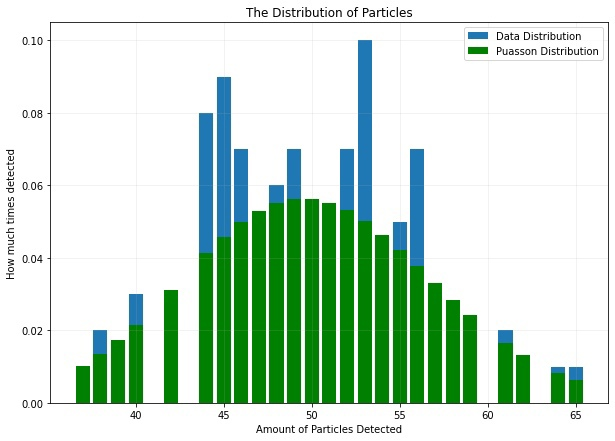
\includegraphics[width=1.0\linewidth]{images/t_40_distribution.jpg}
    \end{figure}
\end{frame}

\begin{frame}{Расчет \chi^2}
        $$\sigma^2 = \frac{\sum\limits_{i=1}^n (\overline{n} - n_i)^2}{n}$$
        $$\sigma_2_0 = 5.9, \;\;\;\; \sqrt{\overline{n}_2_0} = 7.1$$
        
        $$\sigma_4_0 = 4.7,  \;\;\;\; \sqrt{\overline{n}_4_0} = 4.9$$
        $$\chi^2 = \frac{\sum\limits_{i=1}^k ({P_n__i} - w_i)^2}{P_n__i}$$
        $${\chi^2} = 0.10, \;\;\;\; \tau = 20\,s$$
        $${\chi^2} = 0.25, \;\;\;\; \tau = 40\,s$$
\end{frame}

\begin{frame}{\textsc{Расчет} \chi^2}
    сюда высрем распределение хи квадрат для 22 и 23 степеней свободы
\end{frame}

\begin{frame}{\textsc{Измерение с использованием Picoscope 7}}
\begin{figure}
    \centering
    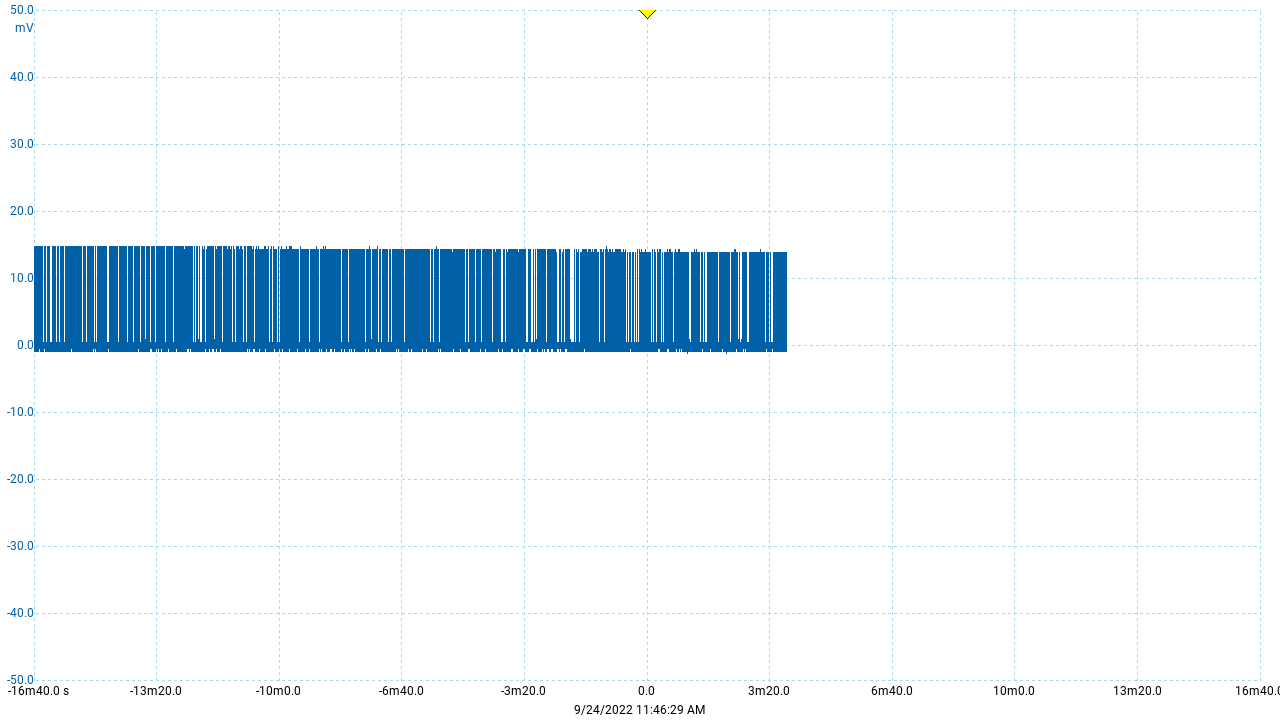
\includegraphics[scale=0.25]{images/Pictrue OF Measures.png}
    \caption{1. Иллюстрация измерений}
    \label{fig:my_label}
\end{figure}
\end{frame}    

\begin{frame}{\textsc{Измерение с использованием Picoscope 7}}
\begin{figure}
    \centering
    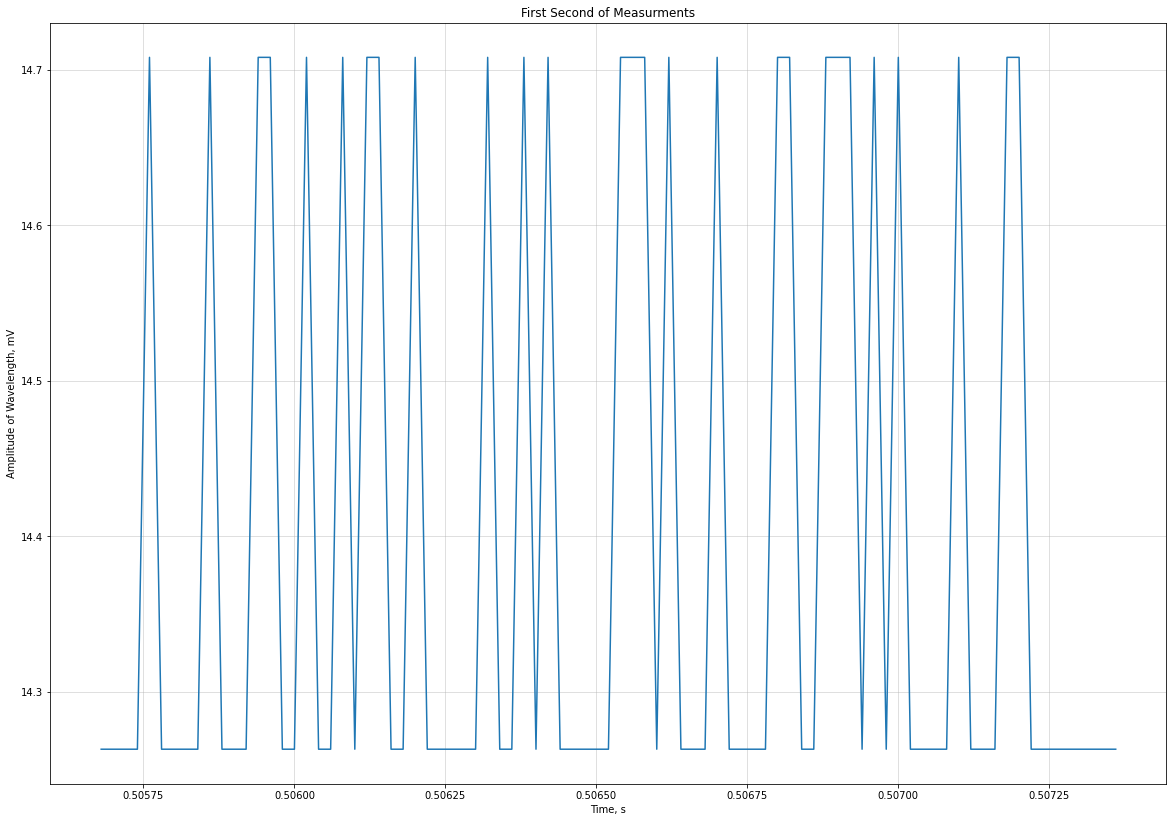
\includegraphics[scale=0.25]{images/outputGraph.png}
    \caption{2. Первая Секунда в Маштабе}
    \label{fig:my_label}
\end{figure}
\end{frame}   

\begin{frame}{\textsc{Измерение с использованием Picoscope 7}}
\begin{figure}
    \centering
    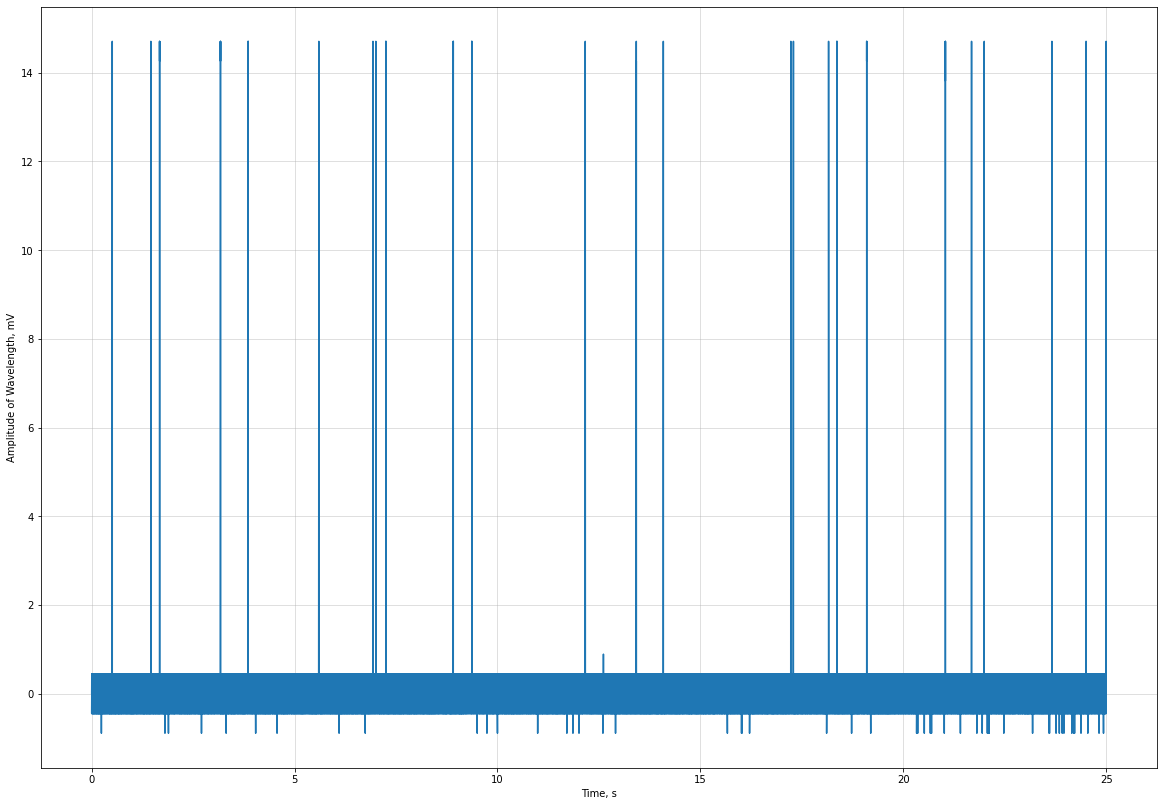
\includegraphics[scale=0.25]{images/outputGraph2.png}
    \caption{3. Промежуток 25 секунд}
    \label{fig:my_label}
\end{figure}
\end{frame}  

\begin{frame}{\textsc{Измерение с использованием Picoscope 7}}
    \large Данные были приведенны в бинарный вид и обработаны с помощью python  
\begin{figure}
    \centering
    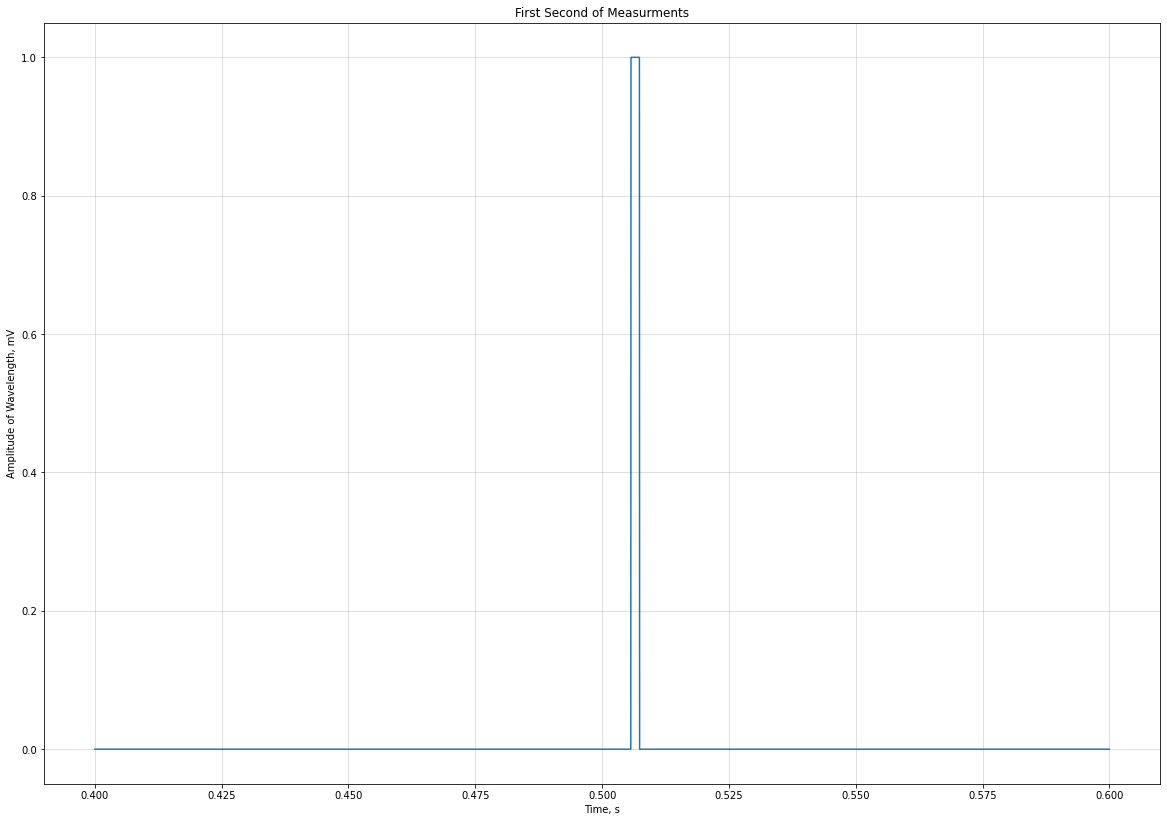
\includegraphics[scale=0.25]{images/outputBin.png}
    \caption{3. Промежуток 25 секунд}
    \label{fig:my_label}
\end{figure}
\end{frame}  


\begin{frame}{\textsc{Измерение с использованием Picoscope 7}}
\begin{figure}
    \centering
    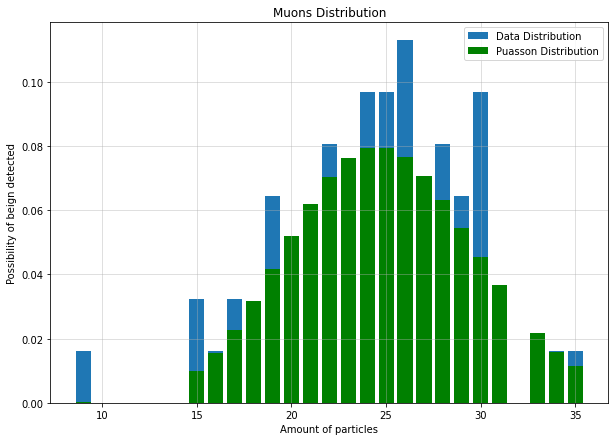
\includegraphics[scale=0.45]{images/outputGraph3.png}
    \caption{4. Распределение данных для 20 секунд}
    \label{fig:my_label}
\end{figure}
\end{frame}  

\begin{frame}{\textsc{Вывод}}
    \large Данные полученные из STAT и с цифрового осциллографа совпадают. Характеристика распределение удовлятворяет распределению Пуассона с точностью \chi^2 - указать
\end{frame}  

\begin{frame}{\textsc{Ссылки}}
    \begin{enumerate}
        \item \href{https://github.com/hK04/LabWorksFIrstSem/tree/main/CosmicRaysRadiation}{Исходнки jupyter notebook с обработкой данных и latex кодом презентации}
    \end{enumerate}
\end{frame}  

\end{document}